%%%%%%%%%%%     INTRODUCCION    %%%%%%%%%%
\chapter{Introducción\label{ch:intro}}

% La biometría se basa en las características biológicas o de comportamiento de un individuo para su identificación \cite{ISO/DefinicionBiometria}. Los sistemas biométricos de identificación se han generalizado de tal manera que es posible encontrarlos desde un dispositivo personal hasta en los cruces de fronteras.

Vivimos en un mundo cada vez más globalizado y al mismo tiempo existe cada vez un mayor interés en \textbf{reforzar las fronteras} y en distinguir entre \textbf{viajeros \textit{legales} e \textit{ilegales}}.

\medskip
\textbf{Pasaportes y fronteras} 
\medskip

Hasta el siglo XV no surge la palabra pasaporte como la combinación de dos palabras francesas (\textit{<<pass>>}, pasar  y \textit{<<porte>>}, puerto o puerta) que se refería al documento en el que se indicaban las ciudades a las que podía acceder un viajero, pero existen, a lo largo de la historia, algunas referencias a otros documentos de viaje. 

El que se considera el primer visado se remonta al año $450$ a.c, cuando \mbox{Artajerjes I} de Persia, emitió un documento que  permitía viajar de forma segura por toda Judea a su lacayo Nehemías. También en la antigua china, durante la dinastía Quing se emitían unos documentos (el \textit{zhuan}) que permitían moverse libremente por todo el territorio imperial. Este documento proporcionaba además del nombre y la edad, ciertas características biométricas que permitían identificar al titular del documento. 

En la Europa medieval los limites entre países eran casi simbólicos y sólo las ciudades de cierta importancia se protegían mediante fortificaciones y murallas que tenían sobretodo un objetivo de defensa militar, pero también permitían a las autoridades de dichas ciudades evitar la entrada de personas no deseadas: Vagabundos, mendigos o enfermos. Por ejemplo, para que los ciudadanos pudieran viajar por las ciudades del califato se requería el \textit{bara'a}, un documento que certificaba su tributación y demostraba que habían pagado sus impuestos.

% Con el crecimiento de las ciudades las fronteras fueron cobrando mayor importancia. Y durante el siglo XV surge la palabra pasaporte como la combinación de dos palabras francesas (\textit{pass}, pasar  y\textit{porte}, puerto o puerta). 

En el siglo XIV aparece la idea moderna de un pasaporte. Enrique V de Inglaterra impone un documento como prueba de ciudadanía permitía el acceso a las ciudades de su reino sin necesidad de pagar las tasas correspondientes. Y a finales del siglo XVIII, durante las guerras jacobinas en Francia, se empleaban pasaportes, o más bien proto-visados que garantizaban la estancia en un determinado país.

Durante el siglo XIX se empezaron a realizar controles de inmigración para acceder a los países, pero fue durante la Primera Guerra Mundial ($1914$) cuando se produjo el verdadero impulso de estos controles y de los pasaportes. Algunos países, como Inglaterra, empezaron a incluir fotografías y descripciones del aspecto de los viajeros para incrementar la seguridad en los cruces de frontera hasta que finalmente la Liga de las Naciones, la actual \GLS{ONU}, en $1920$ estandarizó un formato para los pasaportes europeos. 

% Durante la recensión económica de $1873$ se  empezaron a realizar controles de inmigración para acceder a los países, atendiendo al origen étnico del viajero y a su nacionalidad. Pero no fue hasta la primera guerra mundial hasta que estos controles se hicieron más estrictos. También durante la Primera Guerra Mundial en $1914$ los pasaportes ingleses comenzaron a incluir fotografías y una descripción física del viajero para incrementar la seguridad a raíz de que un espía alemán \textit{Carl Hans Lody} entrará ilegalmente en el país con un pasaporte estadounidense. 

% En $1920$ se puede considerar el nacimiento del pasaporte moderno ya que surgen los primeros pasaportes estandarizados por la liga de las naciones para controlar la emigración a países europeos. 

% Y tuvieron que pasar $60$ años, hasta $1980$ cuando la \textit{International Civil Aviation Organization} (\gls{ICAO}), crea el primer estándar de pasaporte legibles por una máquina.

\begin{figure}[ht]
     \centering
     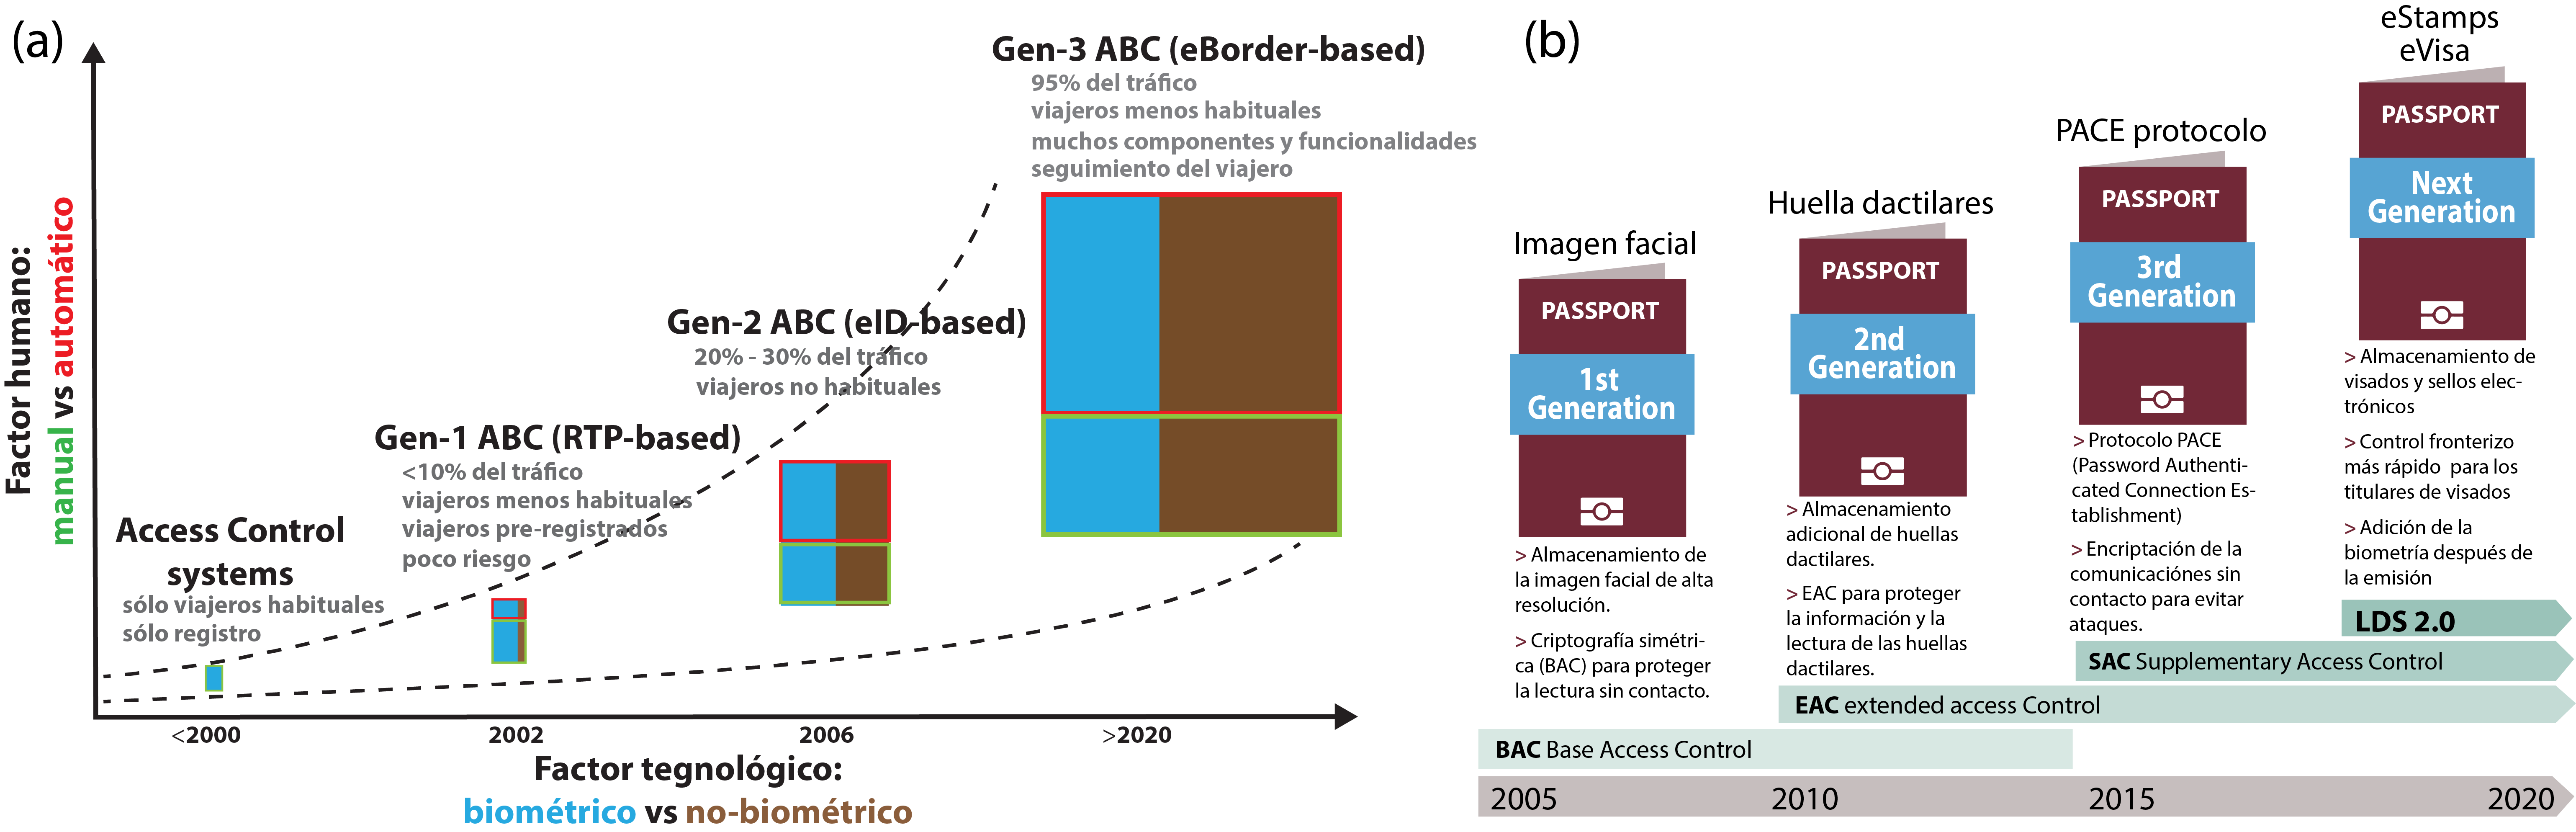
\includegraphics[width=\textwidth]{ch-sistemasABC/images/ch-introduccion/GENEALOGIAS_DE_ABCS_Y_PASAPORTES.png}
     \caption{(a) Evolución de los sistemas \GLS{ABC} y (b) Generaciones para documentos de viaje fijado por \GLS{ICAO}\cite{ICAOOnline}.}
     \label{fig:generacionesABC_Pasaportes}
\end{figure}

A finales del siglo XX se empezaron a buscar formas de automatizar los cruces fronteras. Por ejemplo, en el aeropuerto \textit{Schiphol} de Amsterdam, en $1992$, se empezaron a tomar las huellas dactilares de viajeros frecuentes. Y en $1998$, Malasia, fue el primer país del mundo en emitir pasaportes electrónicos. Pero no fue hasta $2004$, cuando Bélgica lanza el primer pasaporte electrónico adaptado al estándar que un año antes había presentado la \textit{International Civil Aviation Organization} (\gls{ICAO} \cite{ICAOOnline}) para los \textit{Machine Readable Travel Documents} (\gls{MRTD} \cite{doc20069303}). Este estándar es considerado la primera generación de documentos de viaje electrónicos e incluían un circuito integrado con los datos de identificación y la fotografía del titular. A partir de ese momento \GLS{ICAO} ha ido introduciendo mejoras que incrementan las medidas de seguridad. En Fig. \ref{fig:generacionesABC_Pasaportes} (b) se puede ver la evolución de las distintas generaciones de pasaportes electrónicos propuestas por la \GLS{ICAO}.

\medskip
\textbf{Sistemas \GLS{ABC}} 
\medskip

% color{cyan}SECRIP
% En un informe anual publicado por la compañía \textit{Boeing} \cite{BoeingOnline}, la previsión del crecimiento del tráfico de viajeros de aeronaves en todo el mundo alcanza una cantidad de casi el $5$\% en el período $2015$-$2035$ (\cite{Boeing2016}). Este aumento se espera que se duplique hasta el $9,5$\% para el área específica de Asia meridional en el mismo período. Estos números sugieren que se necesita hacer un gran esfuerzo en los próximos años en los controles de seguridad en los puntos de control de fronteras aéreas. Otros tipos de fronteras, como las de
% puertos marítimos y fronteras terrestres, también se espera que sufran de un importante aumento del tráfico \cite{donida2016emerging}.


% Cada día se cruzan millones de fronteras en todo el mundo. Se estima que alrededor de $3,5$ millones de personas cruzaron las fronteras internas entre los países de \textit{\Gls{Schengen}} diariamente en $2017$ \cite{migration2018report}. En el caso de los Estados Unidos, el número de cruces fronterizos en el mismo año fue de aproximadamente $400$ millones \cite{cbp2018snapshot}, mientras que en el Reino Unido se alcanzó la cantidad de $314$ millones \cite{ukborder2017audit} en $2016$.
% \color{black}

% En todos estos cruces fronterizos, los agentes de seguridad tienen que discernir lo antes posible: quién puede o no entrar en el país según las políticas de inmigración o los aspectos de seguridad nacional, si un viajero figura en una lista de sospechosos, actualizar las bases de datos correspondientes o incluso, en algunos casos, sellar el pasaporte del viajero. En conjunto, todas estas operaciones se convierten en una tarea que consume mucho tiempo. De este modo, es necesario dotar a los funcionarios de aduanas y fronteras con procedimientos e instrumentos rápidos y eficaces para garantizar un cómodo cruce de frontera sin colas para los viajero, mientras se mantiene el control del flujo de viajeros. 

Los agentes de frontera deben decidir quién puede pasar al país. Para ello deben tener en cuenta: aspectos de seguridad nacional, políticas de inmigración o si el viajero figura en alguna lista de sospechosos. Además tienen que consultar y actualizar las bases de datos correspondientes y en algunos casos hasta sellar los documentos de viaje. Todas estas tareas consumen mucho tiempo por lo que es necesario dotar a los funcionarios de aduanas y fronteras con procedimientos e instrumentos eficaces para agilizar el tránsito de viajeros. 

En paralelo a la evolución de los documentos de viaje han evolucionado también, los procedimientos y las tecnologías empleadas en los cruces de frontera. Las primeras puertas con lectura de pasaportes se instalaron en Reino Unido, Desde $2008$, y desde entonces los sistemas han ido evolucionando. En los últimos años han surgido los llamados sistemas \textit{Automated Border Control} (\GLS{ABC}). Sistemas automáticos que realizan tres operaciones fundamentales: (1) Autenticación automática de la documentación del viajero, (2) verificación de la identidad de el viajero como titular legítimo de la documentación, mediante procesos biométricos, y (3) Comprobación del permiso para cruzar la frontera atendiendo a las reglas predefinidas. En la figura \ref{fig:generacionesABC_Pasaportes} (a), se observa la evolución de estos sistemas, incrementado la automatización (rojo) frente a los proceso manuales (verde) y también han pasado de ser herramientas de apoyo para los agentes, en la verificación biométrica (azul) a incluir otros procesos, no exclusivamente biométricos (marrón). 

% Todo esto se hace con mínima o ninguna intervención humana \cite{FRONTEX2012OpeReport}.

% (\GLS{ABC}) \cite{del2016automated} para ayudar a las autoridades fronterizas automatizando (totalmente o al menos parcialmente) el proceso. Así, los sistemas \GLS{ABC} se han extendido a todo tipo de fronteras. Los sistemas \GLS{ABC} reducen las habituales molestias de los controles fronterizos y aumentan la satisfacción de los viajeros. Las lineas aéreas y los aeropuertos optimizan sus recursos y los agentes de seguridad pueden centrar su trabajo en las alertas importantes.

% Estos sistemas aumentan el flujo de viajeros a través de la frontera mientras mantienen el control sobre los temas de seguridad. Se basan en documentos de viaje legibles por máquina, como pasaportes, visados, tarjetas de identidad o incluso tarjetas de viajero frecuente. Estos documentos contienen un chip con información como los datos personales del viajero y algunos rasgos biométricos (por ejemplo, el rostro, las huellas dactilares y el iris).


\medskip
\textbf{Sistemas ABC en Europa} 
\medskip

Los sistemas \GLS{ABC} en la Unión Europea (\GLS{EU}) tienen unas características muy especificas. Con la creación del área \Gls{Schengen} en $1995$, se aprobó una nueva política de fronteras para los estados miembros donde sólo se mantuvieron las fronteras exteriores, es decir, con los países fuera del área\footnote{Actualmente, $26$ países europeos pertenecen al área \Gls{Schengen}, de los cuales $4$ no son miembros de la Unión Europea (\GLS{EU}) (Noruega, Islandia, Suiza y Liechtenstein). En un futuro próximo, cuatro miembros más (Bulgaria, Croacia, Chipre y Rumania), estarán obligados a unirse, mientras que los Estados Unidos, Reino Unido e Irlanda han optado por quedarse fuera. También, tres microestados europeos, como Mónaco, San Marino y Ciudad del Vaticano, son miembros de facto. Toda el área \Gls{Schengen} comprende una superficie superior a $4,3$ millones de metros cuadrados y una población de casi $420$ millones de personas,}. Todas las normativas, protocolos y procedimientos para las fronteras en el área \Gls{Schengen} están definidos en \textit{Schengen Borders Code} (\GLS{SBC}) \cite{SBCode2016}. Los viajeros de un estado miembro pueden pasar a otro sin controles fronterizos. Mientras que los viajeros de los estados no miembros, o viajeros de terceros países (\GLS{TCN}), están obligados a cruzar un control fronterizo. Estos Los viajeros pueden encontrarse en dos situaciones legales: los viajeros sin necesidad de un visado (\textit{Third Country Nationals Visa-exempt} (\GLS{TCNVE})), o los que necesitan \gls{visa} o un permiso de residencia (\textit{Third Country Nationals Visa Holders} (\GLS{TCNVH})). Para cada uno de estos tipos de viajeros hay un procedimiento diferente definido en el \GLS{SBC}.

En $2004$ fue fundada la \textit{European Border and Coast Guard Agency} (\Gls{frontex} \cite{FRONTEXOnLine}) con el objetivo de mejorar la gestión de las fronteras exteriores de los estado miembros. 

\medskip
\textbf{Proyecto ABC4EU} 
\medskip
 
Gran parte de los trabajos realizados y las invitaciones presentadas en este documento forma parte de la labor de colaboración llevadas a cabo en el proyecto \GLS{ABC4EU}, 2014 \cite{ABC4EUOnline}. Este proyecto, dentro del Séptimo Programa Marco de la \gls{EU} (\GLS{FP7}), tenia como objetivos mejorar el flujo de trabajo y las funcionalidades de los \GLS{ABC} para todo tipo de fronteras (aeropuertos, puertos y fronteras terrestres) en la \GLS{EU}. Identificar problemas y definir los requisitos de estos sistemas dentro del área \Gls{Schengen}. Varias instituciones de ocho países europeos (Estonia, Finlandia, Alemania, Irlanda, Italia, Portugal, Rumanía, y España) formaron parte del proyecto.

El principal objetivo del proyecto es el diseño de un sistema \GLS{ABC}, cuya prioridad fuera la seguridad, para viajeros \GLS{TCN}, tanto \GLS{TCNVE} como \GLS{TCNVH}. El sistema propuesto debía conformarse a las reglas definidas en \GLS{SBC} ya que manejaba dos importantes bases de datos información sensible \footnote{El proyecto \GLS{ABC4EU} tiene en cuenta la normativa sobre el tratamiento de datos personales de las personas físicas establecido por la \GLS{EU} y por cada país en particular, definido en la directiva $95$/$46$/CE del paramento europeo y del consejo \cite{europea1995directiva}.}: Sistema de Información de Visados (\GLS{VIS}), con información biométrica, y el  \Gls{Schengen} Sistema de Información (\GLS{SIS}) con información sobre actividades delictivas.

\medskip
\textbf{Futuros \Gls{ABC}} 
\medskip

La tendencia indica que los sistemas \GLS{ABC} es separar el proceso en dos etapas: registro y validación. El registro y la validación podrán estar separados para que de esta manera el viajero pueda registrarse de marea previa al viaje.

Los dispositivos \GLS{ABC} en los cruces de frontera tendrán una captura dinámica (\Gls{OnTheFly}) de forma que los viajeros no tengan que detenerse y así agilizar el flujo de viajeros.

\medskip
\textbf{Ataques de presentación} 
\medskip

% El proceso de reconocimiento facial es un reto de identificación biométrica bien conocido debido a las altas tasas de precisión alcanzadas y a la baja intrusión en los sujetos identificados.
% Para abordar el proceso de autenticación facial, hay varios métodos. Algunos de estos enfoques tienen requisitos de seguridad elevados. Un ejemplo es el sistema de control fronterizo automático (\GLS{ABC}), en el que se utiliza el rasgo biométrico para controlar y garantizar el proceso de cruce de fronteras. El proceso de autenticación del \GLS{ABC} tiene que determinar si existe o no coincidencia entre la imagen facial almacenada en el(\GLS{eMRTD}) y una captura \textit{in situ}.

% Los sistemas ABC están expuestos a múltiples ataques o amenazas, por ejemplo, robo de identidad o fraude, lo que también se llama "\textit{\gls{spoofing}}". Por esta razón, muchos trabajos de investigación actuales centran su atención en las técnicas \textit{\gls{antispoofing}} \cite{del2017face}.

% En los últimos años, el amplio uso de los sistemas \GLS{ABC} en los aeropuertos ha aumentado la atención y el estudio de las posibles amenazas múltiples (por ejemplo, el ataque a la presentación) como explica la \textit{European Border and Coast Guard Agency} (\GLS{frontex}) \cite{FRONTEXOnLine}, \cite{FRONTEX2016TechReport}. Estos ataques incentivan la proliferación de algoritmos sobre detección de ataques de presentación (\GLS{PAD}) \cite{jia2019survey}, \cite{ramachandra2017presentation}, \cite{damer2016practical} 

% Millones de pasajeros viajan cada día, siendo el cruce de fronteras una de sus actividades más comunes. En estos puntos es extremadamente importante que la seguridad esté completamente garantizada. Sin embargo, el mantenimiento de niveles de seguridad adecuados es una cuestión muy exigente. Esto ha promovido el desarrollo de sistemas capaces de proporcionar apoyo a las autoridades fronterizas mediante la automatización de algunas de sus tareas. 

Los sistemas \GLS{ABC} se han convertido en una herramienta clave en los cruces de fronteras. Aumentan el flujo de viajeros ya que pueden lograr evaluaciones rápidas de las personas a través de la verificación biométrica de sus documentos \gls{eMRTD}. Sin embargo, esto ha motivado que la aparición de ataques a este tipo de sistemas se haya incrementado notablemente. Los ataques más comunes son los ataques de presentación (\textit{presentation attack} \GLS{PA}) que consisten en la suplantación de la identidad del viajero (\gls{spoofing}). Son relativamente fáciles de llevar a cabo y no requieren un gran conocimiento de la implementación interna del sistema. Paa hacer frente a este tipo de amenazas los \GLS{ABC} se han dotado de métodos \gls{antispoofing} o \textit{Presentation Attack Detection} (\GLS{PAD}).

% Una de las tareas que realizan los sistemas \GLS{ABC} es la identificación biométrica del viajero. Esto se realiza gene ralmente comparando el rostro capturado del sujeto en posición frontal estática con la imagen del rostro almacenada en el pasaporte. Para esta configuración (el sujeto se sitúa delante de la cámara), los sistemas han incluido diferentes algoritmos de Detección de Ataque de Presentación (\GLS{PAD}) (véase, por ejemplo, \cite{ramachandra2017presentation}). Esto ha aumentado su capacidad de detectar diversos tipos de ataques como máscaras, fotos impresas o vídeos en pantalla. En cualquier caso, la mayor parte de la responsabilidad de la detección de ataques recae en los guardias fronterizos que supervisan el sistema.

\medskip
\textbf{Ataques \Gls{morphing}} 
\medskip

El \gls{morphing} es uno de los \GLS{PA} más peligrosos ya que los sistemas biométricos no suelen ser capaces de detectarlos. El \gls{morphing} consiste en fusionar dos imágenes para obtener una imagen intermedia. El proceso de morphing surgió en el mundo de las artes visuales y los efectos especiales, pero al alcanzar tan alto grado de precisión, rápidamente se convirtió en una amenaza para los sistemas biométricos. Cómo \GLS{PA}, en \gls{morphing} consiste en generar una imagen qué combina los rasgos biométricos de varios individuos. Aunque es posible realizar este proceso con distintos rasgos biométricos (iris, huellas dactilares), habitualmente, el \gls{morphing}, se realiza con caras. En los sistemas \gls{ABC}, el ataque de morphing consiste en reemplazar la imagen almacenada en los \gls{eMRTD} de un viajero genuino y reemplazarla por una imagen que mezcla los rasgos genuinos con los de otro individuo impostor, qué tratará de cruzar la frontera con los documentos manipulados.

En los últimos años se han incrementado las investigaciones sobre métodos \GLS{PAD} para detectar ataques \gls{morphing}, estos métodos 
se conocen como métodos \textit{Morphing Attack Detection} (\GLS{MAD}).

% El proceso de \gls{morphing} surgió en el mundo de las artes visuales en películas, vídeos musicales o anuncios, para lograr efectos especiales sorprendentes \cite{lee1998polymorph,ucicr1992feature}. En un principio, el proceso se realizaba manualmente pero rápidamente aparecieron los primeros algoritmos que automatizaron las tareas de \gls{morphing} \cite{wolberg1998image}. Incluso para los expertos resultaba difícil distinguir si una imagen ha sido manipulada mediante \gls{morphing} \cite{beale1995categorical}, \cite{levin2000categorical}, \cite{robertson2018detecting}. Así, la técnica evolucionó de recurso artístico a ser una herramienta delictiva \cite{ferrara2014magic}.

% El \gls{morphing} como ataque de presentación en los sistemas biométricos consiste en generar una imagen mezclando los rasgos de dos sujetos diferentes (el \gls{genuino} y el \gls{impostor}). Comúnmente el \gls{morphing} se realiza con imágenes faciales pero también es posible el \gls{morphing} de otros rasgos biométricos, como el iris \cite{rathgeb2017feasibility} o la huella dactilar \cite{ferrara2016feasibility}.

% En el caso de los sistemas \GLS{ABC} el ataque de \gls{morphing} consiste en manipular la imagen de la cara almacenada en el \textit{chip} del \gls{eMRTD} y reemplazándola por otra que fusiona la identidad del propietario real del documento (que puede o no se cómplice del atacante) y la del viajero \gls{impostor}. En el cruce de fronteras se realiza la comparación de la imagen capturada en el \GLS{ABC} (\textit{vivo}) y la imagen almacenada en el \gls{eMRTD}, entonces, el sistema debe distinguir si el viajero es quien dice ser. La respuesta habitual de esta verificación es la aceptación, teniendo en cuenta la gran similitud entre el rostro del viajero \gls{impostor} y el \gls{morphing} del \gls{eMRTD}.

% Puede considerarse como una de las amenazas más importantes para los sistemas \GLS{ABC} \cite{ramachandra2019towards}, \cite{ferrara2018face}, \cite{makrushin2018overview}, \cite{scherhag2017vulnerability}, \cite{scherhag2020deep}. Se requieren módulos \textit{Morphing Attack Detection} (\GLS{MAD} \cite{scherhag2017vulnerability}, \cite{scherhag2019face}) específicos para la detección de este tipo de ataques presentación.

% En los últimos años se han incrementado las investigaciones sobre \GLS{MAD} e incluso se ha organizado la primera competición \textit{Face Recognition Vendor Test MORPH} del \textit{National Institute of Standards and Technology} (\GLS{NIST}) \cite{frvtMorphOnLine} para tener una visión global y un \textit{ranking} del rendimiento de los algoritmos \GLS{MAD} actuales.


%%%%%%%%%%% OBJETIVOS   %%%%%
\section{Objetivos\label{sec:objetivos}}
% En primer lugar, aborda los sistemas \GLS{ABC} detallando sus configuraciones, diseños posibles y despliegue en entornos reales. A continuación se presentan los ataques de presentación, estableciendo una clasificación básica y describiendo los instrumentos más típicos utilizados para lograrlos. Finalmente, se presentan los sistemas \GLS{PAD}, ilustrando su funcionamiento, evaluando las tecnologías consideradas y sus puntos fuertes y débiles.

Estudiar el estado del arte de los sistemas \GLS{ABC} en general y especialmente en el contexto de la zona \Gls{Schengen}.

Estudiar el estado del arte de los ataques de presentación sistemas biométricos.

Analizar la problemática de los ataques de presentación en los sistemas \GLS{ABC}.

Participar en la puesta en marcha de un sistema \GLS{ABC} en el entorno real de un cruce de fronteras.
 
Señalar los distintos tipos de sistemas \GLS{ABC}.

Estudiar cómo se organiza es un sistema biométrico dentro de los sistemas \GLS{ABC}.
  
Estudiar los puntos débiles del módulo de captura del subsistema biométrico de los sistemas \GLS{ABC}.


Poner a prueba algunos de los algoritmos con mejor rendimiento

Poner a prueba el rendimiento, en un entorno real, DE los algoritmos PAD mejor valorados en la literatura.

Proponer un método de PAD para la ataques de presentación con morphing.

Analizar y evaluar sistema biométrico de verificación facial de un sistema \GLS{ABC} segregado en dos pasos.

Proponer una arquitectura para un módulo de \GLS{PAD} en un sistema \GLS{ABC} captura dinámica.



%%%%% ESTRUCTURA DE LA TESIS %%%%%
\section{Estructura del documentos\label{ch:estructura}}

Este documento se divide en 9 capítulos.

Este primer capítulo presenta una introducción el tema de los sistemas \GLS{ABC} y a la amenaza qué suponen los ataques de presentación para estos sistemas. Además, se detallan los objetivos que busca el presente estudio.

El Capítulo \ref{ch:EstadoDelArte} es una recopilación de un gran número de investigaciones que abordan los temas a tratar en este estudio. Este estado del arte está organizado entre secciones, enfocadas cada una de ellas a un aspecto de la tesis: Sección \ref{sec:estadoArteABC}, sobre sistemas \GLS{ABC}, Sección \ref{sec:estadoArteAtaquesPresentacion}, sobre ataques de presentación y Sección \ref{sec:estadoArteMorphing} centrada en ataques de presentación con \gls{morphing}.

El Capítulo \ref{ch:introSistemasABC} presenta una contextualización de los sistemas \GLS{ABC} en la Sección \ref{sec:sistemasABC} y de los ataques de presentación en la Sección \ref{sec:ContextoAtaquesPresentacion}.

El capítulo \ref{ch:BBDDs} describe cada una de las bases de datos construidas para llevar a cabo los experimentos y las investigaciones realizadas.

El capítulo \ref{ch:PAD_MULTIATAQUE} pone a prueba de alguno de los algoritmos del estado del arte con mejores rendimientos, usando datos capturados por sistema \GLS{ABC} en un entorno real. Y propone un método \GLS{PAD} para hacer frente a diferentes tipos de ataque.

El capítulo \ref{ch:EVALUACIONACION_TOPOLOGIAS} analiza el subsistema biométrico de un sistema \GLS{ABC} de dos etapas segregadas. Además de evaluar la doble verificación características de estos sistemas. Se propone un \GLS{PAD} y se evalúa su rendimiento en ambas capturas.

El capítulo \ref{ch:morphing} expone la problemática de los ataques de presentación con \gls{morphing} y propone un método de \GLS{PAD} para la detección de este tipo de ataques.

El Capítulo \ref{ch:ABC_OnTheFly} expone la problemática de los ataques de presentación en sistemas \GLS{ABC} con captura dinámica (\Gls{OnTheFly}). Y propone una arquitectura para un módulo \GLS{PAD} que sea adapta a este tipo de sistemas.

El capítulo \ref{ch:conclusion} presenta las conclusiones extraídas con cada una de las investigaciones presentadas en los capítulos anteriores y las contribuciones que cada una de ellas aposta.
